\section{Methodology}
The system is split into 2 main phases: The Rule Learner (RL) and the Strategy Learner (SL).This is to encapsulate the idea of human-inspired learning that our technique focuses on. Figure \ref{fig:sys_arch} outlines the System Architecture. The RL receives the game board (in this case, Connect4) as an input and starts playing randomly against the game. In this case, the learner is only concerned about making valid moves and not actually winning the game. This again, is how a human would start learning Connect4 when given the game to play for the first time without any prior instructions. Once the system learns the rules of the game, they are given to the SL along with the board as input. The SL then starts playing against the game adhering to the given rules and tries to learn the optimal winning strategy. The following subsections go into further details on how the RL and SL are implemented.

\begin{figure}
  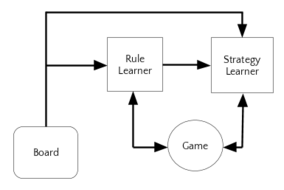
\includegraphics[width=\linewidth]{sys_arch.png}
  \caption{The system architecture with the computational flow.}
  \label{fig:sys_arch}
\end{figure}

\subsection{Rule Learner}
The Rule Learner’s task is to return the valid moves given a certain board state. The board is represented by a $H$X$W$X$3$ tensor, where $H$ and $W$ are the board height and width while the third dimension is used to represent the state of each grid cell. This tensor encodes the state of each of the h x w board cells, which can be:
\begin{itemize}
 \item Empty
 \item Occupied by player 1
 \item Occupied by player 2
\end{itemize}
These states are encoded by the vectors [1 0 0], [0 1 0] and [0 0 1] respectively.

The output is represented by a $H$X$W$ matrix. Valid moves are indicated by the respective elements in the matrix having been set to 1. Non-valid moves are represented by 0s.
The RL network maps the input tensor to the output matrix. The network has an input layer with $H$X$W$X$3$ units, a single 50-unit fully-connected hidden layer with a $tanh$ activation function, and a fully connected $tanh$ output layer with $H$X$W$ units. More information about the train and test process is given in section 3.

\subsection{Strategy Learner}
Similiar to DeepMind we used a convolutional neural network to train the Strategy Learner. This network consists of an input layer which takes in the state of the board and the valid moves from the rule learner. This then goes to a single convolution layer with filters of size 4 by 4. From there we enter into a fully connected layer with 64 nodes and finally to the output layer with 7 nodes, 1 for each column. A graphical representation of the network can be seen in Figure \ref{fig:strat_learn}.

\begin{figure}
  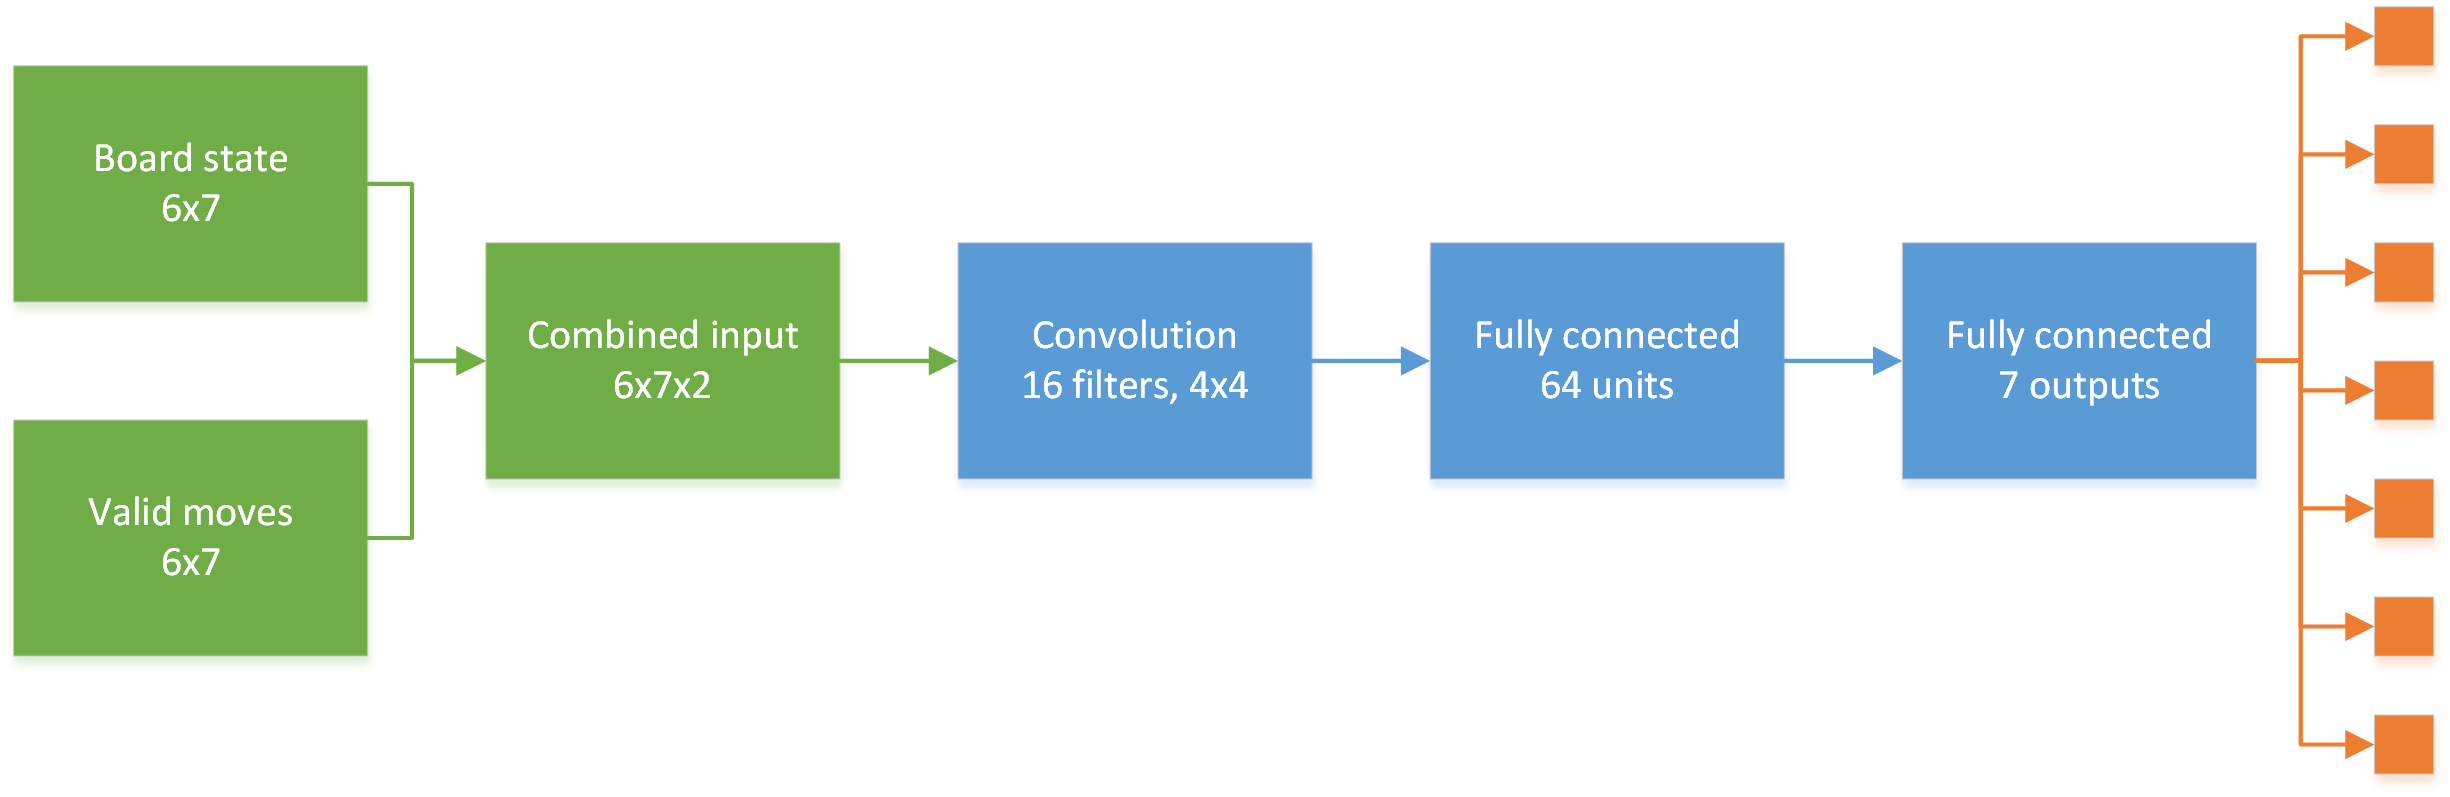
\includegraphics[width=\linewidth]{Network1.png}
  \caption{Strategy Learner network structure}
  \label{fig:strat_learn}
\end{figure}
